%%   $ sudo apt-get install texinfo
%%   $ texi2pdf -c lecture.tex

\PassOptionsToPackage{table}{xcolor}
\documentclass[pdf]{beamer}
\mode<presentation>{\usetheme{Dresden}}
\usepackage{lmodern}
\usepackage{amsmath,textcomp,amssymb,geometry,graphicx,listings,array,color,amsthm}

\usepackage{tikz}
\usepackage{multicol}
\usetikzlibrary{shapes,snakes}
\usetikzlibrary{positioning}
\usetikzlibrary{arrows}
\usetikzlibrary{fit}

%% For on-slide alerting of nodes
\tikzstyle{alert} = [text=black, fill=blue!20, draw=black]
\setbeamercolor{alerted text}{fg=blue}
\tikzset{alerton/.code args={<#1>}{%
  \only<#1>{\pgfkeysalso{alert}} % \pgfkeysalso doesn't change the path
}}

%% utils for removing uninteresting sections from the navbar
%% https://tex.stackexchange.com/questions/317774/hide-section-from-sidebar
\makeatletter
\let\beamer@writeslidentry@miniframeson=\beamer@writeslidentry%
\def\beamer@writeslidentry@miniframesoff{%
  \expandafter\beamer@ifempty\expandafter{\beamer@framestartpage}{}% does not happen normally
  {%else
    % removed \addtocontents commands
    \clearpage\beamer@notesactions%
  }
}
\newcommand*{\miniframeson}{\let\beamer@writeslidentry=\beamer@writeslidentry@miniframeson}
\newcommand*{\miniframesoff}{\let\beamer@writeslidentry=\beamer@writeslidentry@miniframesoff}
\makeatother

%% preamble
\title{Auto-Differentiation}
\subtitle{At the Intersection of Nifty and Obvious}
\author{A.C.}
\date{\today}

\AtBeginSection[]
{
  \miniframesoff
  \begin{frame}{Outline}
  \tableofcontents
  \end{frame}
  \miniframeson
}

\definecolor{darkred}{rgb}{0.7,0,0}
\definecolor{darkgreen}{rgb}{0,0.5,0}
\definecolor{darkblue}{rgb}{0,0,0.5}
\definecolor{darkpurple}{rgb}{0.4, 0.0, 0.4}

%% Code font settings
\lstset{
  showstringspaces=false,
  basicstyle=\scriptsize\ttfamily,
  commentstyle=\color{darkred},
  stringstyle=\color{darkgreen},
  keywordstyle=\bfseries\color{darkpurple},
}

%%%%%%%%%%%%%%%%%%%%%%%%%%
% Start of Actual slides %
%%%%%%%%%%%%%%%%%%%%%%%%%%
\begin{document}
\begin{frame}
  \titlepage
\end{frame}

%% Quick reminder total and partial derivatives, gradients, Jacobians, and most
%% importantly, the flow-chart simplicity of derivatives.
\section{Derivatives Refresher}
\begin{frame}{Univariate Derivatives}
  \begin{itemize}
  \item The instantaneous rate of change of $f$ in response to infinitesimal
    perturbations in $x$.
  \item The slope of the tangent line through $(x,f(x))$.
  \end{itemize}
  \pause
  \begin{definition}
    Let $f:\mathbb{R}\rightarrow\mathbb{R}$. We say that $f$ is differentiable
    wherever the limit

    \[ f' = \lim_{h \rightarrow 0} \frac{f(x+h)-f(x)}{h} \]

    exists and we call $f'$ the derivative of $f$.
  \end{definition}
\end{frame}

\begin{frame}{Derivatives of Transformations}
  Linearity: \[(\alpha f+ \beta g)' = \alpha f' + \beta g'\]
  \pause
  Product rule: \[(fg)' = f'g + fg'\]
  \pause
  Quotient rule: \[\left(\frac{f}{g}\right)' = \frac{f'g - fg'}{g^2}\]
  \pause
  Chain rule: \[(f \circ g)' = g' \cdot (f' \circ g)\]
\end{frame}

\begin{frame}{Gradients}
  \begin{itemize}
  \item Lots of interesting functions operate on multiple inputs.
  \pause
  \item Idea: take the derivative with respect to one input at at time.
    \begin{itemize}
    \item Pretend the other inputs don't exist, or rather, are constant.
    \item Collate it all into a vector at the end.
    \end{itemize}
  \end{itemize}
  \pause
  \begin{definition}
    Let $f:\mathbb{R}^n\rightarrow\mathbb{R}$, and $u_i$ be the $i$th Cartesian
    unit vector in $\mathbb{R}^n$. We say that $f$ is differentiable wherever
    the limit

    \[ \frac{\partial f}{\partial x_i} = {\nabla f}_i = \lim_{h \rightarrow 0} \frac{f(x + hu_i)-f(x)}{h} \]

    exists for all $i \in [1,n]$. We call $\nabla f$ the gradient of $f$.
  \end{definition}
\end{frame}

\begin{frame}{Jacobians}
  \begin{itemize}
  \item Some functions have multiple outputs, too.
  \item Similar trick:
    \begin{itemize}
    \item Compute the gradient for each output
    \item Glue the gradients to one another
    \item Give the resulting matrix a fancy name
    \end{itemize}
  \end{itemize}
  \pause
  \begin{definition}
    Let $f:\mathbb{R}^n\rightarrow\mathbb{R}^m$, be differentiable in each of its outputs at $x$. We define the Jacobian of $f$ to be the matrix such that

    \[ J_{ij} = \frac{\partial f_i}{\partial x_j} \]
  \end{definition}
\end{frame}

%% Detailed description of autodiff algorithms.
\section{Autodiff}
\subsection{Key Insight}
\begin{frame}{First Piece}
  \begin{itemize}
  \item Differentiation is a flowchart.
    \begin{itemize}
    \item An \emph{easy} flowchart: \url{https://xkcd.com/2117/}
    \end{itemize}
  \pause\item Flowcharts are programs.
  \end{itemize}
\end{frame}

\begin{frame}{Second Piece}
  \begin{itemize}
  \item Numerical programs may include loops, branches, etc
    \begin{itemize}
    \item Not always easy to express in closed form
    \end{itemize}
  \pause
  \item But when it executes it has to boil down to some finite composition of
    ALU-executable operations.
    \begin{itemize}
    \item We know how to differentiate sums, products, differences, etc
    \end{itemize}
  \end{itemize}
\end{frame}

\begin{frame}{Eureka}
  \begin{itemize}
  \item Apply the ``differentiation flowchart'' to the composite function defined by
  the \emph{execution} of a numerical program.
  \pause
  \item Compute $J_f(x)$ at the same time as $f(x)$!
  \end{itemize}
\end{frame}

\subsection{Forward Mode}
\begin{frame}{Dependent Variables}
  \begin{itemize}
  \item Many intermediate calculations in most computer programs.
  \pause
  \item Treat intermediate calculations as anonymous dependent variables.
  \pause
  \item Keep track of every dependent variable's gradient WRT inputs.
    \begin{itemize}
    \item Propagate forward with product rule, quotient rule, etc.
    \end{itemize}
  \pause
  \item Use independent variables to bootstrap the calculation
    \begin{itemize}
    \item $\frac{\partial x_i}{\partial x_j} = I_{i=j}$
    \end{itemize}
  \end{itemize}
\end{frame}

\begin{frame}{Dep Vars Example}
  Consider the function $f(x,y) = x^2y + 2y$, and let

  \begin{flalign*}
  & g_1 = x \cdot x   \implies \nabla g_1 = x \cdot (1, 0)^T + (1, 0)^T \cdot x \\
  \uncover<2->{ & g_2 = g_1 \cdot y \implies \nabla g_2 = g_1 \cdot (0, 1)^T + \nabla g_1 \cdot y \\}
  \uncover<3->{ & g_3 = 2y          \implies \nabla g_3 = 2 \cdot (0, 1)^T \\}
  \uncover<4->{ & f = g_2 + g_3     \implies \nabla f = \nabla g_2  + \nabla g_3 \\}
  \end{flalign*}
  \uncover<4->{Exercise for the reader: confirm that $\nabla f = (2xy, x^2 + 2)^T$}
\end{frame}

\begin{frame}[fragile]{Code I}
\begin{lstlisting}[language=Python]
class _FDepVar(object):
    def __init__(self, val, grad):
        self.val = val
        self.grad = grad

    def __add__(f, g):
        if not isinstance(g, _FDepVar):
            return _FDepVar(f.val + g, f.grad)
        return _FDepVar(f.val + g.val, f.grad + g.grad)

    def __mul__(f, g):
        if not isinstance(f, _FDepVar):
            return _FDepVar(f.val*g, f.grad*g)
        return _FDepVar(f.val*g.val,
                        f.grad*g.val + f.val*g.grad)
\end{lstlisting}
\end{frame}

\begin{frame}[fragile]{Code II}
\begin{lstlisting}[language=Python]
def forward(f):
    def f_J(*args):
        wrapped = []
        for i, arg in enumerate(args):
            grad = np.zeros(len(args))
            grad[i] = 1
            wrapped.append(_FDepVar(arg, grad))
        out = f(*wrapped)
        try:
            return ([o.val for o in out],
                    [o.grad for o in out])
        except TypeError:
            return out.val, out.grad
    return f_J
\end{lstlisting}
\end{frame}

\begin{frame}{Caveats}
  \begin{itemize}
  \item Every scalar operation in our program now a vector op
  \item Calculation is $n$ times more expensive, where $n$ is our number of
    inputs.
    \begin{itemize}
    \item No big deal for auto-diffing $f(x,y,z)$
    \item But if $f$ takes thousands of parameters \ldots\ hoo boy
    \end{itemize}
  \end{itemize}
\end{frame}

\subsection{Backward Mode}
\begin{frame}{Key Idea}
  \begin{itemize}
  \item Derivatives don't have to be taken WRT input variables
  \pause
  \item Forward mode: take $\frac{dg}{dx}, \frac{dh}{dx}$, build $\frac{df}{dx}$
    \begin{itemize}
    \item Derivatives of different functions with respect to $x$
    \end{itemize}
  \pause
  \item Backward mode: take $\frac{df}{dg}, \frac{df}{dh}$, build $\frac{df}{dx}$
    \begin{itemize}
    \item Derivatives of $f$ with respect to different variables.
    \item Multivariate chain rule is central:
      \[ \frac{df(g(x),h(x))}{dx} = \frac{\partial f}{\partial g} \cdot \frac{dg}{dx} + \frac{\partial f}{\partial h} \cdot \frac{dh}{dx} \]
    \end{itemize}
  \end{itemize}
\end{frame}

\begin{frame}{Calculation Graph}
  Calculations naturally form a DAG as they feed into one another:
\begin{center}
  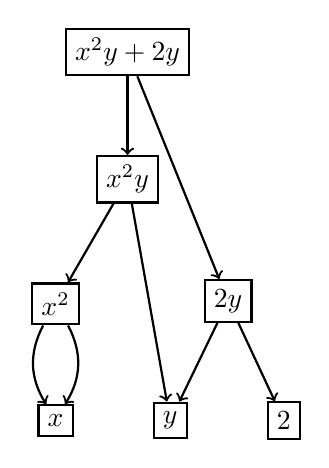
\begin{tikzpicture}[thick,auto,->]
  \uncover<1->{
    \node[alerton={<1>}] (x)[draw=black] {$x$};}
  \uncover<1->{
    \node[alerton={<1>},right = of x] (y)[draw=black] {$y$};}
  \uncover<1->{
    \node[alerton={<1>},right = of y] (two)[draw=black] {$2$};}
  \uncover<2->{
    \node[alerton={<2>},above = of x] (x2)[draw=black] {$x^2$};}
  \uncover<3->{
    \node[alerton={<3>},above right = 1 and 0.2 of x2] (x2y)[draw=black] {$x^2y$};}
  \uncover<4->{
    \node[alerton={<4>},above right = 1 and 0.2 of y] (2y)[draw=black] {$2y$};}
  \uncover<5->{
    \node[alerton={<5>},above = of x2y] (f)[draw=black] {$x^2y + 2y$};}

  \uncover<2->{
    \path (x2) edge[bend left] (x);
    \path (x2) edge[bend right] (x);}
  \uncover<3->{
    \path (x2y) edge (x2);
    \path (x2y) edge (y);}
  \uncover<4->{
    \path (2y) edge (two);
    \path (2y) edge (y);}
  \uncover<5->{
    \path (f) edge (x2y);
    \path (f) edge (2y);}
\end{tikzpicture}
\end{center}
\end{frame}

\begin{frame}{Edge Weights}
  Edges provide a convenient place to record our various
  $\frac{\partial g_i}{\partial g_j}$s:
\begin{center}
  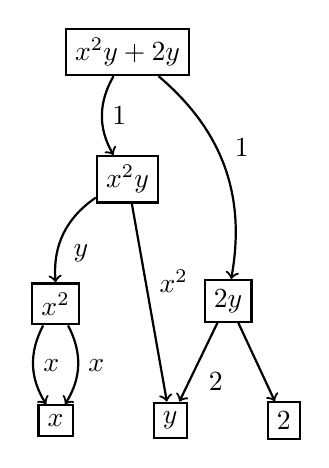
\begin{tikzpicture}[thick,auto,->]
  \uncover<1->{
    \node[] (x)[draw=black] {$x$};}
  \uncover<1->{
    \node[right = of x] (y)[draw=black] {$y$};}
  \uncover<1->{
    \node[right = of y] (two)[draw=black] {$2$};}
  \uncover<1->{
    \node[above = of x] (x2)[draw=black] {$x^2$};}
  \uncover<2->{
    \node[above right = 1 and 0.2 of x2] (x2y)[draw=black] {$x^2y$};}
  \uncover<3->{
    \node[above right = 1 and 0.2 of y] (2y)[draw=black] {$2y$};}
  \uncover<4->{
    \node[above = of x2y] (f)[draw=black] {$x^2y + 2y$};}

  \uncover<1->{
    \path (x2) edge[bend left] node {$x$} (x);
    \path (x2) edge[bend right] node {$x$} (x);}
  \uncover<2->{
    \path (x2y) edge[bend right] node {$y$} (x2);
    \path (x2y) edge node {$x^2$} (y);}
  \uncover<3->{
    \path (2y) edge (two);
    \path (2y) edge node {$2$} (y);}
  \uncover<4->{
    \path (f) edge[bend right] node {1} (x2y);
    \path (f) edge[bend left] node {1} (2y);}
\end{tikzpicture}
\end{center}
\end{frame}

\begin{frame}{Propagation}
  \begin{itemize}
  \item If we know all of $\frac{df}{d\text{parent}}$,
    then by the chain rule $\frac{df}{d\text{self}}$ is just the weighted sum
    of its parents.
    \begin{itemize}
    \item Root node always knows its derivative: $\frac{df}{df} = 1$
    \end{itemize}
    \pause
  \item Note: DAG-order traversal, not just a DFS.
    \begin{itemize}
    \item we can't visit a node until all its parents are done.
    \item we have to traverse all edges, not visit every node.
    \end{itemize}
  \end{itemize}
\end{frame}

\begin{frame}{Propagation Example}
\begin{center}
  \begin{tikzpicture}[thick,auto,->]
  \uncover<1->{
    \node[] (x)[draw=black] {
      {\only<-4>{0}}%
      {\only<5->{$2xy$}}%
    };}
  \uncover<1->{
    \node[right = of x] (y)[draw=black] {
      {\only<1-2>{0}}%
      {\only<3>{2}}%
      {\only<4->{$x^2 + 2$}}%
    };}
  \uncover<1->{
    \node[right = of y] (two)[draw=black,fill=black] {2};}
  \uncover<-4>{
    \node[above = of x] (x2)[draw=black] {
        {\only<-3>{0}}%
        {\only<4->{$y$}}%
    };}
  \uncover<-3>{
    \node[above right = 1 and 0.2 of x2] (x2y)[draw=black] {
      {\only<1>{0}}%
      {\only<2->{1}}%
    };}
  \uncover<-2>{
    \node[above right = 1 and 0.2 of y] (2y)[draw=black] {
      {\only<1>{0}}%
      {\only<2>{1}}%
    };}
  \uncover<-1>{
    \node[above = of x2y] (f)[draw=black] {1};}

  \uncover<-4>{
    \path (x2) edge[bend left] node {$x$} (x);
    \path (x2) edge[bend right] node {$x$} (x);}
  \uncover<-3>{
    \path (x2y) edge[bend right] node {$y$} (x2);
    \path (x2y) edge node {$x^2$} (y);}
  \uncover<-2>{
    \path (2y) edge (two);
    \path (2y) edge node {$2$} (y);}
  \uncover<-1>{
    \path (f) edge[bend right] node {1} (x2y);
    \path (f) edge[bend left] node {1} (2y);}
\end{tikzpicture}
\end{center}
\end{frame}

\begin{frame}{Code}
  \begin{itemize}
  \item The code for backward mode is a little less slide-deck friendly than for
    forward mode, so we'll skip it here.
  \item A (crude) implementation is available in this presentation's git
    repository for those interested in perusing it.
  \end{itemize}  
\end{frame}

\begin{frame}{Caveats}
  \begin{itemize}
  \item Have to propagate derivatives backward for every output.
    \begin{itemize}
    \item Calculation is $m$ times more expensive, where $m$ is our number of
      outputs.
    \end{itemize}
    \pause
  \item Have to remember the calculation graph.
    \begin{itemize}
    \item Requires additional space proportional to the length of the
      computation.
    \end{itemize}
  \end{itemize}
\end{frame}

%% Application of autodiff to loss optimization, and therefore to ML.
\section{A Practical Application}
\begin{frame}{Disclaimer}
  \emph{ACHTUNG}: Aggressive, true-from-10k-feet-but-not-below-that simplifications
  ahead.
\end{frame}
  
\begin{frame}[fragile]{ML $\approx$ Optimization}
  \begin{itemize}
  \item Most ML boils down to one of
    \begin{itemize}
    \item Classification: Find me the best decision boundary for all this the
      training data I've marked as positive or negative.
    \item Regression: Find me the function that best matches these data points I
      measured.
    \end{itemize}
    \pause
  \item If we define a loss function $\mathcal{L}$, and model parameters
    $\theta$ for tuning it, and call our training data $X, Y$, then we
    can formulate them as
    \[ \arg\min_{\theta} \mathcal{L}(X,Y;\theta) \]
    \begin{itemize}
    \item E.g. in linear regression, $\mathcal{L} = ||X^T\theta - y||_2^2$
    \end{itemize}
  \end{itemize}
\end{frame}

\begin{frame}{Gradient Descent in a Nutshell}
  \begin{itemize}
  \item When you're on a hill and want to get to the bottom, \emph{walk downhill}.
    \pause
  \item The gradient of your loss function tells you which way is downhill.
      \[ \theta_n = \theta_{n-1} - h_n \nabla \mathcal{L}(\theta_{n-1}) \]
  \end{itemize}
\end{frame}

\begin{frame}{Neural Networks \& Backpropagation}
  \begin{itemize}
  \item Neural Networks are commonly optimized (trained) using gradient descent.
    \pause
  \item But formulating the gradient is a PITA, sure would be nice if we could
    generate the gradient at a point programmatically and efficiently \ldots
    \pause
  \item Which is exactly what autodiff does.
    \begin{itemize}
    \item Neural networks have many, many parameters to train on, but we only
      have one loss function, so backward mode is a no-brainer.
    \item Frequently called backpropagation or backprop for historical reasons.
    \end{itemize}
  \end{itemize}
\end{frame}

%% Q&A and Further reading.
\miniframesoff
\section*{}
\begin{frame}{References and Additional Materials}
  \begin{itemize}
  \item The source for this presentation is hosted at
    \url{https://github.com/alan-christopher/autodiff-edu}.
  \item A recorded presentation of this slide deck can be found at
    \url{https://youtu.be/Fntkxhcs3mU}
  \end{itemize}
\end{frame}

\begin{frame}{Questions?}
\end{frame}
\end{document}
